\documentclass[../report.tex]{subfiles}
\begin{document}

\graphicspath{{img/}{../img/}}

\section{Product Breakdown}

Et product breakdown diagram laves ved at se p� et helt projekt og finde ud af hvilke dele det best�r af. Man inddeler alts� projektet i produkter som n�r de bliver sat sammen vil udg�re et f�rdigt projekt. Hvert produkt kan s� deles ind i mindre produkter, ligesom man g�r med hele projektet. Produkterne vil p� den m�de danne et hierarki hvor det �verste produkt vil v�re hele projektet og de nederste produkter vil v�re detaljerede produkter som er mere h�ndgribelige.\\

\noindent
Ved at lave et product breakdown diagram f�r man et bedre overblik over, hvad der skal laves for at projektet bliver f�rdigt. Senere i projektet kan man ogs� bruge det til at holde styr p� om alle dele af projektet er blevet lavet.\\

\noindent
I target-projektet blev der lavet et product breakdown diagram med relativt f� produkter. Det er med andre ord ikke blevet brudt ned i meget detaljerede produkter. Selve product breakdown diagrammet blev prim�rt brugt i starten af projektet, til at f� et overblik hvad der skulle laves. Men det blev ogs� brugt som basis for at lave et activity breakdown diagram.
 
\newgeometry{left=5cm,bottom=3cm}
\begin{landscape}

\subsection{Product Breakdown Diagram}

\begin{figure}[H]

\label{fig:Product Breakdown Diagram}
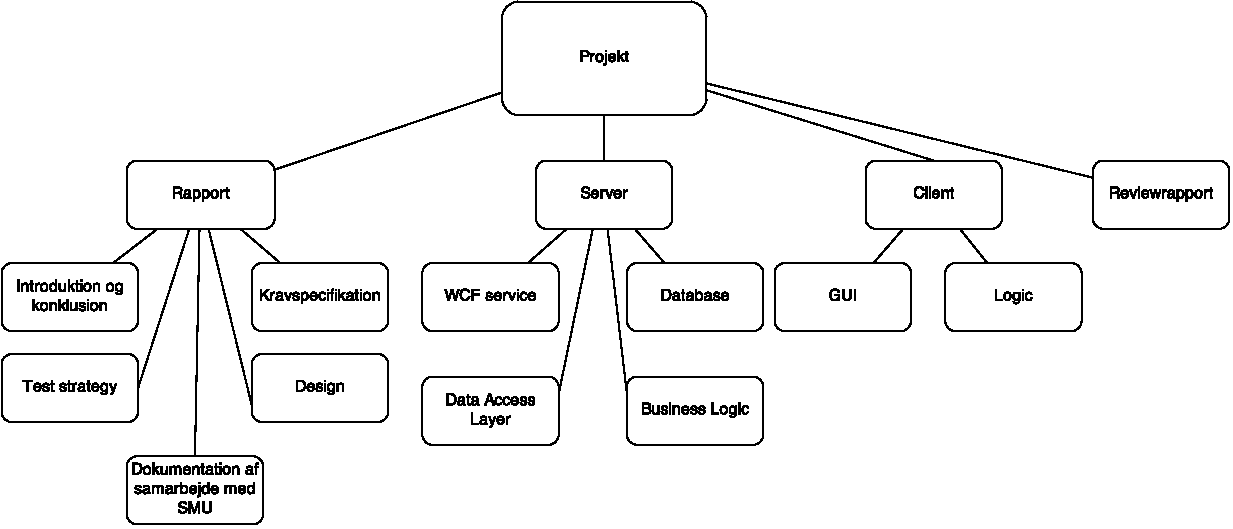
\includegraphics[ scale=1]{ProductBreakdownDiagram.pdf}
\caption{Product Breakdown Diagram}

\end{figure}

\end{landscape}

\end{document}